\chapter{Example accident model}
\label{ch:accident_model}
Using FRAM restrospectively will, hopefully, identify some of the critically constrained couplings between functions in a system. Appling this knowlegde, it will be possible not only to build safer, but also more resillient system.\\
\\
This chapter will take a relevant near-miss and model it with the procedure suggested by FRAM. 

\section{Near miss at Train crossing}
Modelling a near miss incident is not very common, though very rewarding in terms of drawing experience from them. A more elaborate explanation of what a near miss is, see section \ref{sec:near_miss}

%Previous studies\cite{belmonte2011interdisciplinary}

\subsection{Background}
At Grenåbanen tuesday the 26th of March 2010, at 14:40, an ambulance was intentionally led over railway crossing that should have been secured. This situation led to a near-miss, and luckily no one was harmed.

\subsubsection{Official accident report}
Train RV 4940 in transit from Grenå towards Aarhus was signalled that crossing 128a was secured.

Shortly after, the train driver realized that 2 railway employees were located on the track. The driver did not do anything further as he assumed they would move when they saw the train.

As the train approached the crossing, an ambulance with siren signal entered the crossing - from the road side. The train driver used the emergency brake, hereby avoiding collision with the ambulance. According the the train driver, the collision was imminent.\\
\\
The 2 railway employees reported that, they though they would be able to assist the ambulance in reaching its destination faster, by leading it into the crossing before the train arrived, by misjudged the situation.\\
\\
The document ``udrykningsbekendtgørelsen'' (the official notice regarding emergency) states that the driver of an emergency vehicle, must at all times abide signals or other instructions, at railway crossings

Following the initial investigations and evaluations of the data available - the accident investigation committee reached the following conclusion; further studies would not necessarily lead to preventative recommendations, or result in findings leading to significant improvements in railway safety.

With reference to Danish railway legislation, the accident investigation committee decided not to perform further studies. 

\subsection{Assumptions}
As there are only crossing bars in the driving direction - it is assumed that the crossing bars were in place as the event took place. Figure \ref{fig:ambulance_path} illustrates the assumed path of the ambulance and the placement of the crossing bars.
\begin{figure}
 \centering
   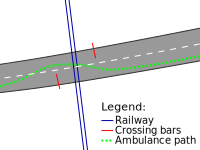
\includegraphics[width=150pt]{figures/accident_overview.pdf}
 \caption{Assumed ambulance path}
 \label{fig:ambulance_path}
\end{figure}

\subsubsection{FRAM model}
TODO

Functions: 
Signal

(Crossing bar)


\subsubsection{Functions}
\begin{table}[h]
\centering
    \begin{tabular}{ | l | r | }
    \hline
    Function     &  Block passage from road side\\ \hline \hline
    Input        &  \\ \hline
    Output       &  Lower the crossing bars\\ \hline
    Precondition &  Signal the car drivers\\ \hline
    Resource     &  \\ \hline
    Time         &  Drivers have been notified\\ \hline
    Control      &  Train has passed\\ \hline
    \end{tabular}
\caption{Function 1}
\label{table:function}
\end{table}

\begin{table}[h]
\centering
    \begin{tabular}{ | l | r | }
    \hline
    Function     &  Allow passage from train side \\ \hline \hline
    Input        &  Train has enters crossing\\ \hline
    Output       &  Train has left crossing\\ \hline
    Precondition &  Crossing bars a lowered\\ \hline
    Resource     &  \\ \hline
    Time         &  Must pass within blocking-time window\\ \hline
    Control      &  Road side passage blocked\\ \hline
    \end{tabular}
\caption{Function 1}
\label{table:function0}
\end{table}

\begin{table}[h]
\centering
    \begin{tabular}{ | l | r | }
    \hline
    Function     &  Signal train allowed passage \\ \hline \hline
    Input        &  \\ \hline
    Output       &  \\ \hline
    Precondition &  \\ \hline
    Resource     &  \\ \hline
    Time         &  \\ \hline
    Control      &  \\ \hline
    \end{tabular}
\caption{Function 1}
\label{table:function1}
\end{table}

\begin{table}[h]
\centering
    \begin{tabular}{ | l | r | }
    \hline
    Function     &  Unblock road side \\ \hline \hline
    Input        &  Train has left crossing\\ \hline
    Output       &  \\ \hline
    Precondition &  \\ \hline
    Resource     &  \\ \hline
    Time         &  \\ \hline
    Control      &  \\ \hline
    \end{tabular}
\caption{Function 1}
\label{table:function2}
\end{table}


\begin{figure}[h]
 \centering
   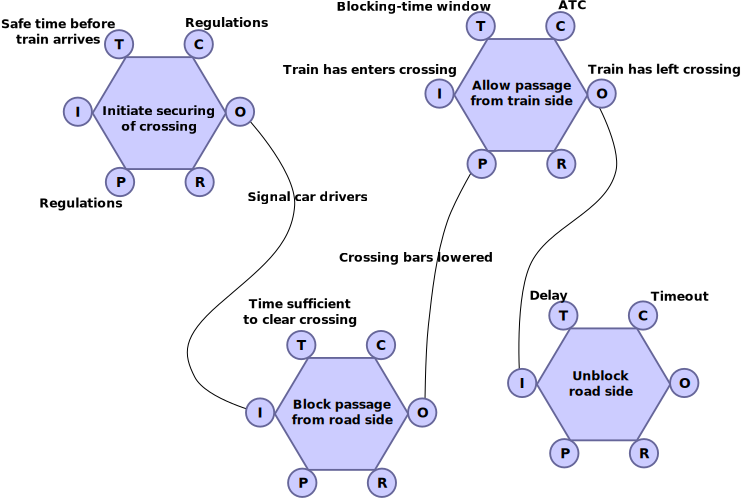
\includegraphics[width=1\textwidth]{figures/Accident_fram_model.pdf}
 \caption{Graphical FRAM representation}
 \label{fig:fram_graphical}
\end{figure}

This approach treats the train as the product input and outputs.

\subsection{Barriers}
There is a physical barrier that is intercoupled with a incorporeal barrier; the crossing bars that depend on driving in the right side of the road (following traffic laws).
There are two overall incorporeal barriers in place here; ``udrykningsbekendtgørelsen'' and the railway legislation.
\section{Discussion}
%TODO In general, like in statistics, Corrolation does not imply causation.

The near-miss her is beyond the scope of the intended operation/design of ATC(\ref{sec:atc}). This is a perfect example of high variability in a system. Everything works as intended, until the railway workers are affected by a disturbance that ultimately leads to two time constraint pressures; one from the Ambulance, and one from the approaching train.

On the remedial side, there could be a gain by adding a second set of barriers, meaning that both driving lanes of the road will be blocked. This will prevent this barrier to be overridden entirely.

%TODO The fields usabilty engineering and safety enginering are closely related in terms of clear communication.